\documentclass[12pt, a4paper]{article}
\usepackage{amsmath, amsthm, amssymb, appendix, bm, graphicx, hyperref, mathrsfs,fancyhdr,ctex,nameref,tikz}

% 定义新的页眉样式
\fancypagestyle{sectionheader}{
    \fancyhf{} % 清空当前页眉设置
	\fancyhead[L]{Page:\thepage}
	%\fancyhead[C]{中间页眉}
	\fancyhead[R]{\leftmark}
}
\setlength{\headheight}{14.49998pt}
\addtolength{\topmargin}{-2.49998pt}


\numberwithin{equation}{section} % 每个节开始时重新编号公式
\title{Assignment2}
\author{PhilFan}
\date{\today}
\linespread{1.5}



\begin{document}

\maketitle
\setcounter{page}{0}
\maketitle
\thispagestyle{empty}



%目录页
\newpage
\pagenumbering{Roman}
\setcounter{page}{1}
\tableofcontents

%第一节
\newpage
\setcounter{page}{1}
\pagenumbering{arabic}
\pagestyle{sectionheader} % 使用自定义的页眉样式

\section{不可压缩Navier-Stokes方程}
\label{sec:a}
二维不可压缩流体的流场完全由速度向量 $q = (u(x, y), v(x, y))\in \mathbb{R^2} $和压力 $p(x, y) \in \mathbb{R} $描述。这些函数是以下守恒定律的解 ~\cite{refa}:

\begin{itemize}
    \item 质量守恒:
\end{itemize}
\begin{equation}
div(q) = 0,
\end{equation}或者用散度算子\footnote{
这里我们回顾一下二维场中v散度、梯度和拉普拉斯算子的定义:y
如果 $v = (v_x,v_y): \mathbb{R^2} \mapsto \mathbb{R^2}$,$\varphi:\mathbb{R^2} \mapsto \mathbb{R}$则
\begin{equation}
div(v) = \frac{\partial v_x}{\partial x} + \frac{\partial v_y}{\partial y}, \quad 
\mathscr{G}_\varphi = (\frac{\partial \varphi}{\partial x} , \frac{\partial \varphi}{\partial y}),\quad
\Delta{\varphi}   =  \frac{\partial ^2 \varphi}{\partial x^2} + \frac{\partial ^2 \varphi}{\partial y^2},\quad \\ and\quad\Delta{v}   =  (\Delta{v_x},\Delta{v_y}).
\notag
\end{equation}} 的显式形式表示为:
\begin{equation}
\frac{\partial u}{\partial x} + \frac{\partial v}{\partial y} = 0
\label{eq:div}
\notag
\end{equation}
\begin{itemize}
    \item 动量守恒方程的紧凑形式\footnote{我们用$\otimes$ 表示张量积。}:
\end{itemize}
\begin{equation}
\frac{\partial q}{\partial t} + div(q\otimes q) = -\mathscr{G}p + \frac{1}{Re} \Delta q 
\end{equation}
或者显式形式为:
\begin{equation}
\left\{
\begin{aligned}
\frac{\partial u}{\partial t} + \frac{\partial ^2 u}{\partial x}+ \frac{\partial uv}{\partial y} = -\frac{\partial p}{\partial x} + \frac{1}{Re} (\frac{\partial ^2 u}{\partial x^2}+\frac{\partial ^2 u}{\partial y^2})\\
\frac{\partial v}{\partial t} + \frac{\partial uv}{\partial x}+ \frac{\partial ^2 v}{\partial y} = -\frac{\partial p}{\partial y} + \frac{1}{Re} (\frac{\partial ^2 v}{\partial x^2}+\frac{\partial ^2 v}{\partial y^2})\\
\end{aligned}
\right.
\label{eq:ns}
\end{equation}




上述方程是以无量纲形式书写的,使用以下缩放变量:
\begin{equation}
x = \frac{x^{\ast}}{L},y = \frac{y^{\ast}}{L},u = \frac{u^{\ast}}{V_0},v=\frac{v^{\ast}}{V_0},t =\frac{t^{\ast}}{L/{V_0}},p =\frac{p^{\ast}}{\rho_0 V_0^2}
\end{equation}
其中上标$(\ast)$ 表示以物理单位测量的变量。常数 $L$ 和 $V_0 $分别是表征模拟流动的参考长度和速度。维数无关数 $Re$ 称为雷诺数,用于量化流动中惯性项(或对流项)和粘性项(或扩散项)之间的相对重要性\footnote{在第一章中讨论了描述对流和扩散现象的模型标量方程。}:

\begin{equation}
Re = \frac{V_0L}{\nu}
\end{equation}

其中$\nu$ 是流体的运动粘度。

总结来看,在这个项目中将通过数值方法求解的Navier-Stokes PDE系统由
%\ref{eq:div}和\ref{eq:ns}
定义;初始条件$(t = 0)$ 时和边界条件将在下面的部分讨论。




%第二节
\newpage
\section{计算域、交错网格和边界条件}
\label{sec:b}
通过考虑一个带周期边界条件的矩形域$ L_x \times L_y$(见\ref{img::left}),数值求解Navier-Stokes方程大大简化了。速度$ q(x, y) $和压力$ p(x, y) $在整个区域上的周期性可以数学地表示为:
\begin{equation}
\begin{aligned}
q(0, y) &= q(L_x, y),p(0, y) = p(L_x, y),\forall y \in \left[ 0,L_y\right] \\
q(x, 0) &= q(x, L_y),p(x, 0) = p(x, L_y),\forall x \in  \left[0, L_x\right] \\
\end{aligned}
\end{equation}

\begin{figure}[htbp]
  \centering
  \begin{minipage}[b]{0.45\textwidth}
    \centering
    \fbox{
      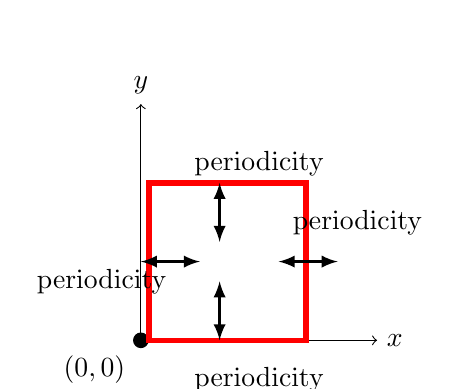
\begin{tikzpicture}[scale=1]
        % 绘制坐标轴
        \draw[->] (0,0) -- (3,0) node[right] {$x$};
        \draw[->] (0,0) -- (0,3) node[above] {$y$};
        % 标注原点和轴名称
        \node[circle,fill,inner sep=2pt,label=below left:{$(0,0)$}] at (0,0) {};

        % 绘制正方形
        \draw[red, line width=2pt] (0.1,0) rectangle (2.1,2);

        % 标注实心箭头和文字
        \draw[latex-latex, line width=1pt, fill=black] (0,1) -- (0.75,1);
        \node at (-0.5,0.75) {periodicity};

        \draw[latex-latex, line width=1pt, fill=black] (1,0) -- (1,0.75);
        \node at (1.5,-0.5) {periodicity};

        \draw[latex-latex, line width=1pt, fill=black] (1,2) -- (1,1.25);
        \node at (1.5,2.25) {periodicity};

        \draw[latex-latex, line width=1pt, fill=black] (2.5,1) -- (1.75,1);
        \node at (2.75,1.5) {periodicity};
      \end{tikzpicture}
    }
    \caption{Pic1}
    \label{img::left}
  \end{minipage}
  
  %\hfill%空隙
  
  \begin{minipage}[b]{0.45\textwidth}
    \centering
    \fbox{
      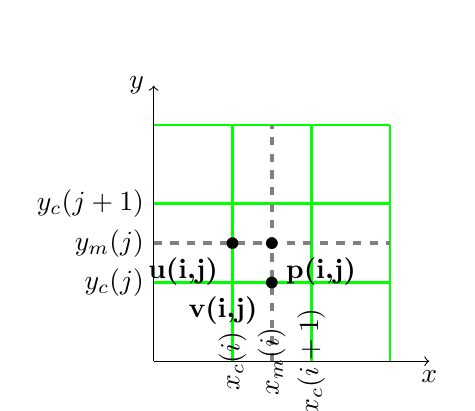
\begin{tikzpicture}[scale=1]
        % 绘制坐标轴
        \draw[->] (0,0) -- (3.5,0) node[below] {$x$};
        \draw[->] (0,0) -- (0,3.5) node[left] {$y$};

        % 绘制网格线
        \foreach \x in {1,2,3}
          \draw[green, line width=1pt] (\x,0) -- (\x,3);
        \foreach \y in {1,2,3}
          \draw[green, line width=1pt] (0,\y) -- (3,\y);

        % 绘制虚线
        \draw[dashed, gray, line width=1.5pt] (1.5,0) -- (1.5,3);
        \draw[dashed, gray, line width=1.5pt] (0,1.5) -- (3,1.5);

        % 标注点
        \node[circle,fill,inner sep=1.5pt,label={[font=\bfseries]below left:\textbf{u(i,j)}}] at (1,1.5) {};
        \node[circle,fill,inner sep=1.5pt,label={[font=\bfseries]below right:\textbf{p(i,j)}}] at (1.5,1.5) {};
        \node[circle,fill,inner sep=1.5pt,label={[font=\bfseries]below left:\textbf{v(i,j)}}] at (1.5,1) {};

        % 标注刻度
        \node[rotate=90] at (1,0) {$x_c(i)$};
	\node[rotate=90] at (1.5,0) {$x_m(i)$};
	\node[rotate=90] at (2,0) {$x_c(i+1)$};

        \node[left] at (0,1) {$y_c(j)$};
        \node[left] at (0,1.5) {$y_m(j)$};
        \node[left] at (0,2) {$y_c(j+1)$};
      \end{tikzpicture}
    }
    \caption{Pic2}
    \label{img::right}
  \end{minipage}
\end{figure}


解将被计算的点按照矩形均匀的二维网格分布在域中。由于不是所有变量在我们的方法中共享相同的网格,我们首先定义一个主要网格(见\ref{img::right},沿着 $x$ 方向取 $n_x$ 个计算点,沿着$y$ 方向取$ n_y $个计算点:
\begin{equation}
\begin{aligned}
x_c(i) = (i - 1)\delta x, \quad \delta x &= \frac{L_x}{n_x - 1},\quad i = 1,..., n_x \\
y_c(j) = (j - 1)\delta y,\quad \delta y &= \frac{L_y}{n_y - 1},\quad j = 1,..., n_y  \\
\end{aligned}
\end{equation}



次要网格由主要网格单元的中心定义:
\begin{equation}
\begin{aligned}
x_m(i) &= (i - 1/2)\delta x,\quad i = 1,...,n_{xm},\\
y_m(j) &= (j - 1/2)\delta y,\quad j = 1,...,n_{ym},\\
\end{aligned}
\end{equation}
其中我们使用了简写符号 $n_{xm} = n_x - 1$,$n_{ym} = n_y - 1$。在计算单元内部,定义为矩形区域 $\left[x_c(i),x_c(i + 1)\right] \times \left[y_c(j), y_c(j + 1)\right]$,未知变量 $u$、$v$、$p$ 将作为在不同空间位置的解的近似值计算:
\begin{itemize}
    \item $u(i, j) \approx u(x_c(i), y_m(j))$(单元的西侧面),
    \item $v(i, j) \approx v(x_m(i), y_c(j))$(单元的南侧面),
    \item $p(i, j) \approx p(x_m(i), y_m(j))$(单元的中心)。
\end{itemize}

这种交错排列的变量排列具有压力和速度之间强耦合的优点。它还有助于避免在共位排列(所有变量都在相同的网格点上计算)中遇到的稳定性和收敛性问题(参见本章末尾的参考文献)。
\newpage
% 使用 Bibtex 文献管理
\bibliographystyle{plain}
\bibliography{references}

\end{document}


